\begin{table}[H]
\centering
\caption{Índices de Sobol e coeficientes de erro correspondentes para análise de
  sensibilidade com 70.000 parametrizações.}
\label{apptab1}
\begin{tabular}{l|r|r|r|r|}
\cline{2-5}
                                                        & \cellcolor[HTML]{C0C0C0}S1 & \cellcolor[HTML]{C0C0C0}S1\_conf & \cellcolor[HTML]{C0C0C0}ST & \cellcolor[HTML]{C0C0C0}ST\_conf \\ \hline
\multicolumn{1}{|l|}{\cellcolor[HTML]{EFEFEF}N}         & 0.004881                   & 0.006388                         & 0.022210                   & 0.003495                         \\ \hline
\multicolumn{1}{|l|}{\cellcolor[HTML]{EFEFEF}n\_issues} & 0.186464                   & \cellcolor[HTML]{FFFFFF}0.025251 & 0.234629                   & 0.014013                         \\ \hline
\multicolumn{1}{|l|}{\cellcolor[HTML]{EFEFEF}p}         & 0.063561                   & 0.015413                         & 0.115790                   & 0.009160                         \\ \hline
\multicolumn{1}{|l|}{\cellcolor[HTML]{EFEFEF}\(\sigma\)}         & 0.462022                   & 0.035358                         & 0.576110                   & 0.029141                         \\ \hline
\multicolumn{1}{|l|}{\cellcolor[HTML]{EFEFEF}\(\rho\)}         & 0.129280                   & 0.018281                         & 0.242048                   & 0.016394                         \\ \hline
\multicolumn{1}{|l|}{\cellcolor[HTML]{EFEFEF}p\_intran} & 0.000949                   & 0.004267                         & 0.011563                   & 0.001754                         \\ \hline
\end{tabular}
\vspace{0.1cm}
\source{Marcelo Veloso Maciel, 2018.}
\end{table}


\begin{table}[H]
\centering
\caption{Índices de Sobol  de segunda ordem (S2 ) para análise de
  sensibilidade com 70.000 parametrizações.}
\label{apptab2}
\begin{tabular}{l|r|r|r|r|r|r|}
\cline{2-7}
                                                        & \cellcolor[HTML]{C0C0C0}N & \cellcolor[HTML]{C0C0C0}n\_issues & \cellcolor[HTML]{C0C0C0}p & \cellcolor[HTML]{C0C0C0}\(\sigma\) & \cellcolor[HTML]{C0C0C0}\(\rho\) & \cellcolor[HTML]{C0C0C0}p\_intran \\ \hline
\multicolumn{1}{|l|}{\cellcolor[HTML]{EFEFEF}N}         & NaN                       & 0.001927                          & 0.002175                  & 0.006913                  & 0.000713                  & 0.000511                          \\ \hline
\multicolumn{1}{|l|}{\cellcolor[HTML]{EFEFEF}n\_issues} & NaN                       & NaN                               & 0.003479                  & 0.002571                  & 0.029061                  & 0.007587                          \\ \hline
\multicolumn{1}{|l|}{\cellcolor[HTML]{EFEFEF}p}         & NaN                       & NaN                               & NaN                       & 0.021056                  & 0.009098                  & 0.002245                          \\ \hline
\multicolumn{1}{|l|}{\cellcolor[HTML]{EFEFEF}\(\sigma\)}         & NaN                       & NaN                               & NaN                       & NaN                       & 0.043554                  & 0.005111                          \\ \hline
\multicolumn{1}{|l|}{\cellcolor[HTML]{EFEFEF}\(\rho\)}         & NaN                       & NaN                               & NaN                       & NaN                       & NaN                       & -0.006991                         \\ \hline
\multicolumn{1}{|l|}{\cellcolor[HTML]{EFEFEF}p\_intran} & NaN                       & NaN                               & NaN                       & NaN                       & NaN                       & NaN                               \\ \hline
\end{tabular}
\vspace{0.1cm}
\source{Marcelo Veloso Maciel,2018.}
\end{table}



\begin{figure}[H]
  \centering
  \caption{Gráfico de dispersão e regressões polinomiais para 70.000 parametrizações.}
    \begin{subfigure}[b]{0.49\textwidth}
        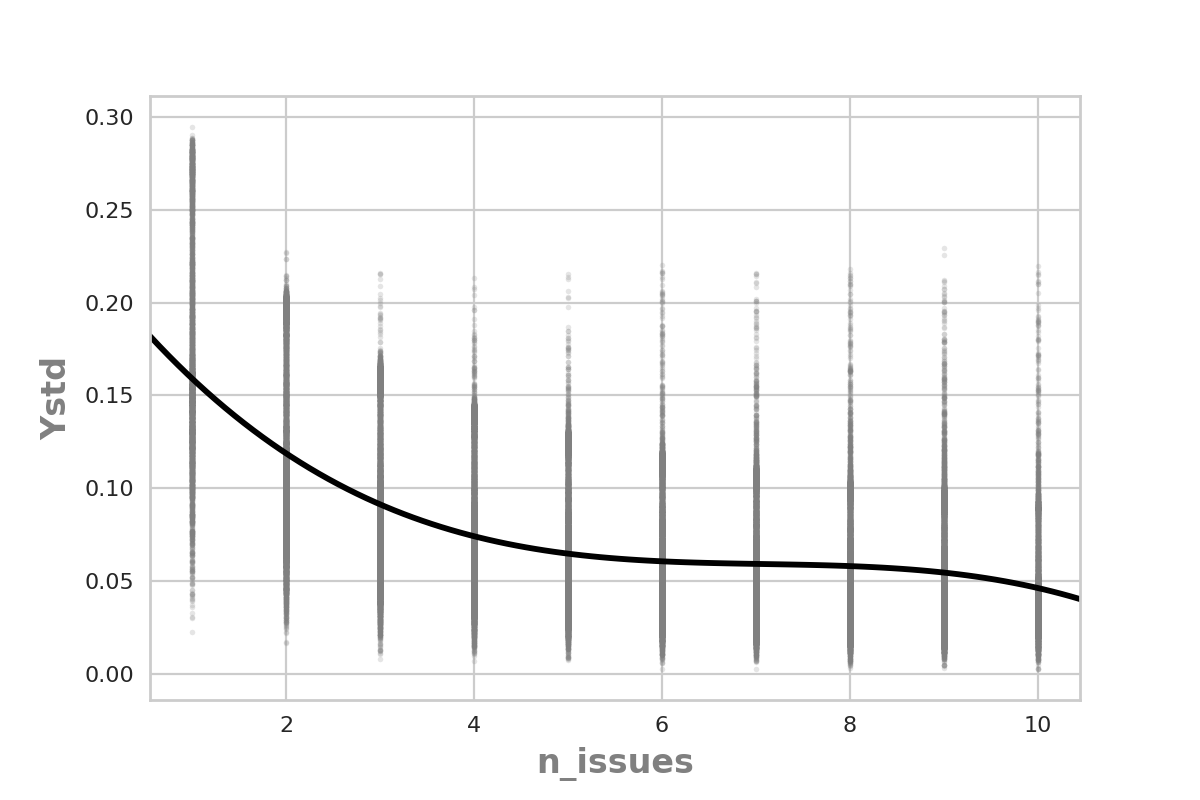
\includegraphics[width=\textwidth]{ims/nlregressions/nlregressionmutatingon_issues.png}
    \end{subfigure}
    \begin{subfigure}[b]{0.49\textwidth}
        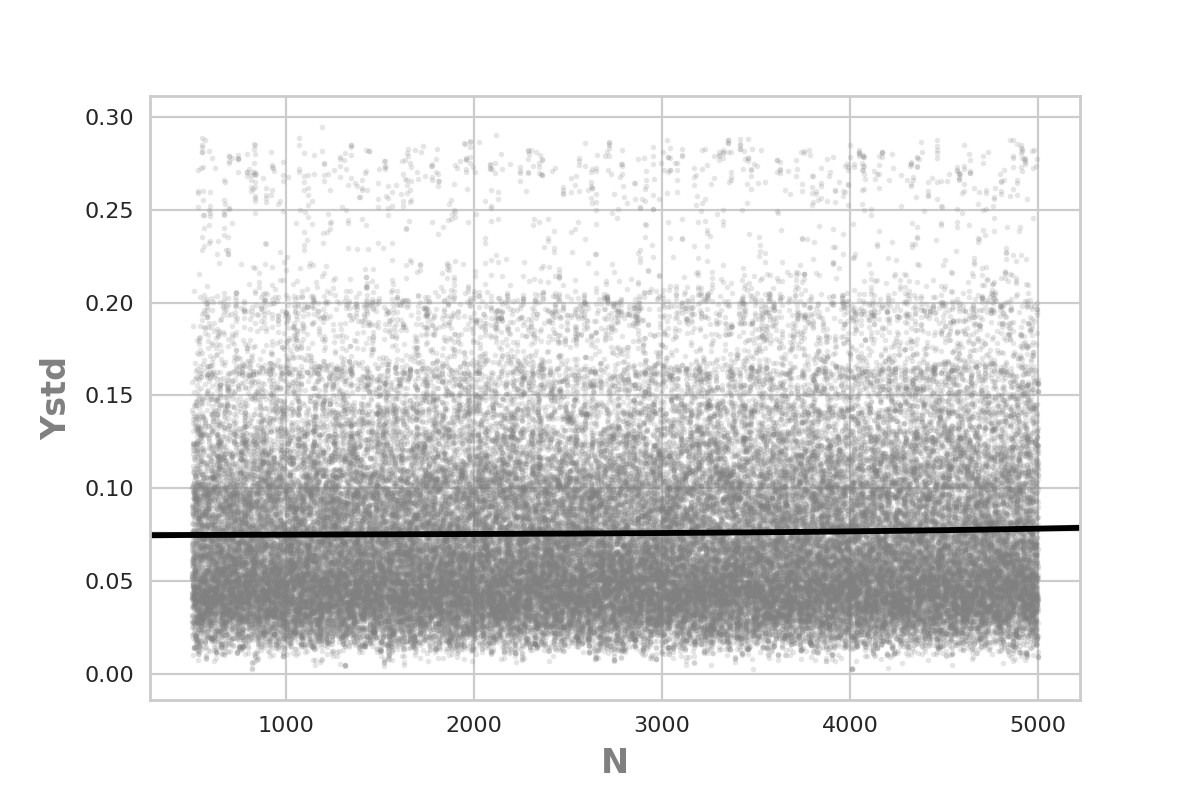
\includegraphics[width=\textwidth]{ims/nlregressions/nlregressionmutatingoN.png}
    \end{subfigure}

    \begin{subfigure}[b]{0.49\textwidth}
        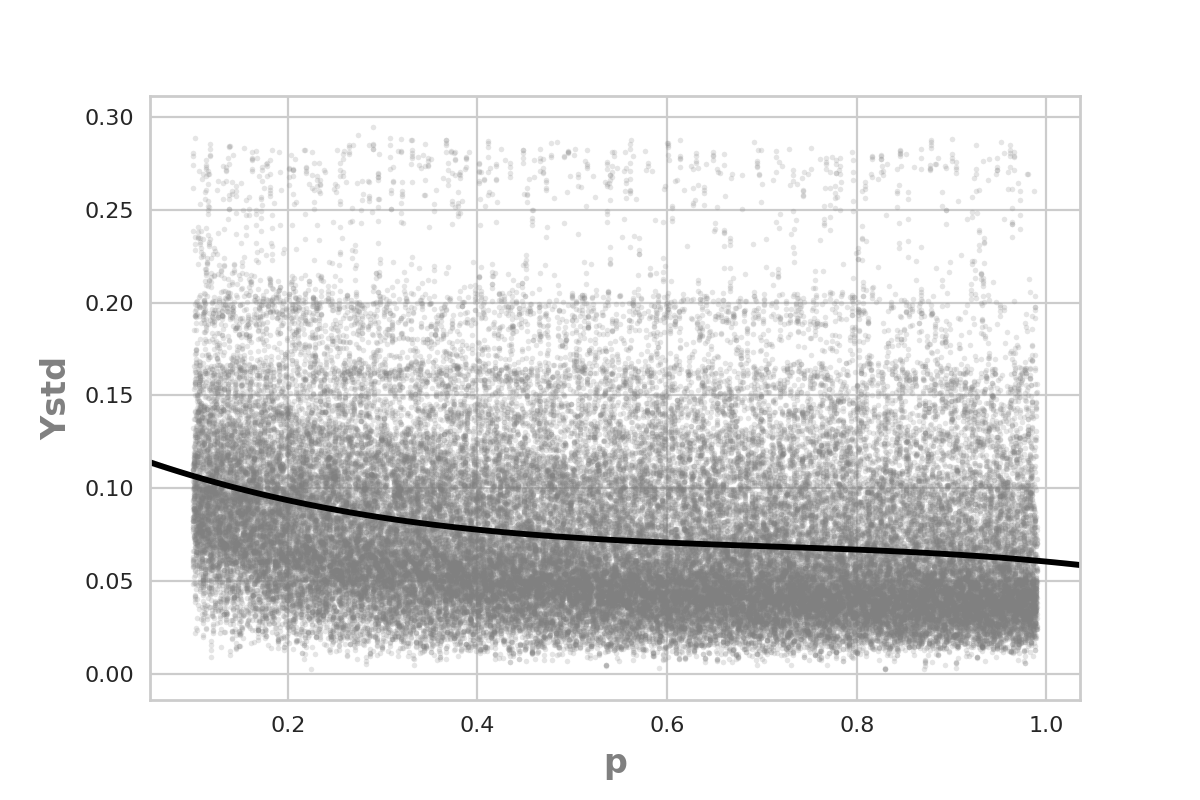
\includegraphics[width=\textwidth]{ims/nlregressions/nlregressionmutatingop.png}
      \end{subfigure}
          \begin{subfigure}[b]{0.49\textwidth}
            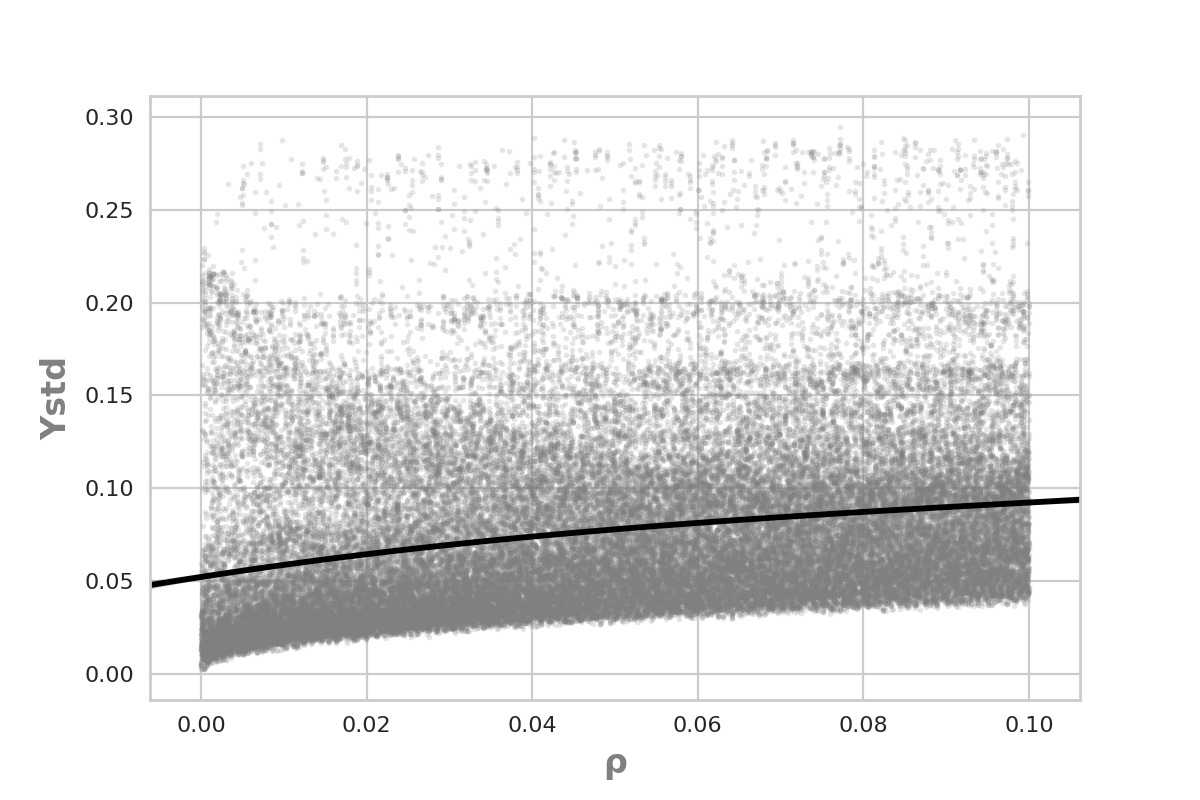
\includegraphics[width=\textwidth]{ims/nlregressions/nlregressionmutatingorho.png}
      \end{subfigure}

                \begin{subfigure}[b]{0.49\textwidth}
            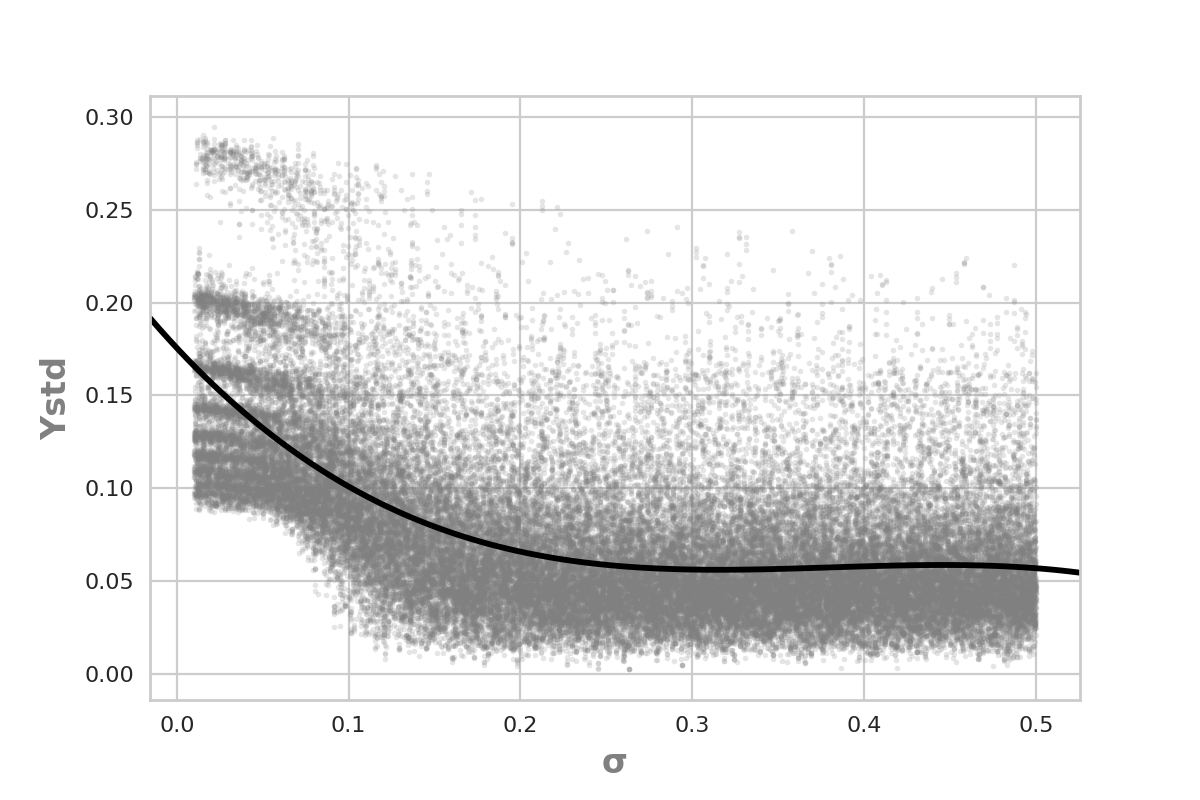
\includegraphics[width=\textwidth]{ims/nlregressions/nlregressionmutatingosigma.png}
          \end{subfigure}
                \begin{subfigure}[b]{0.49\textwidth}
            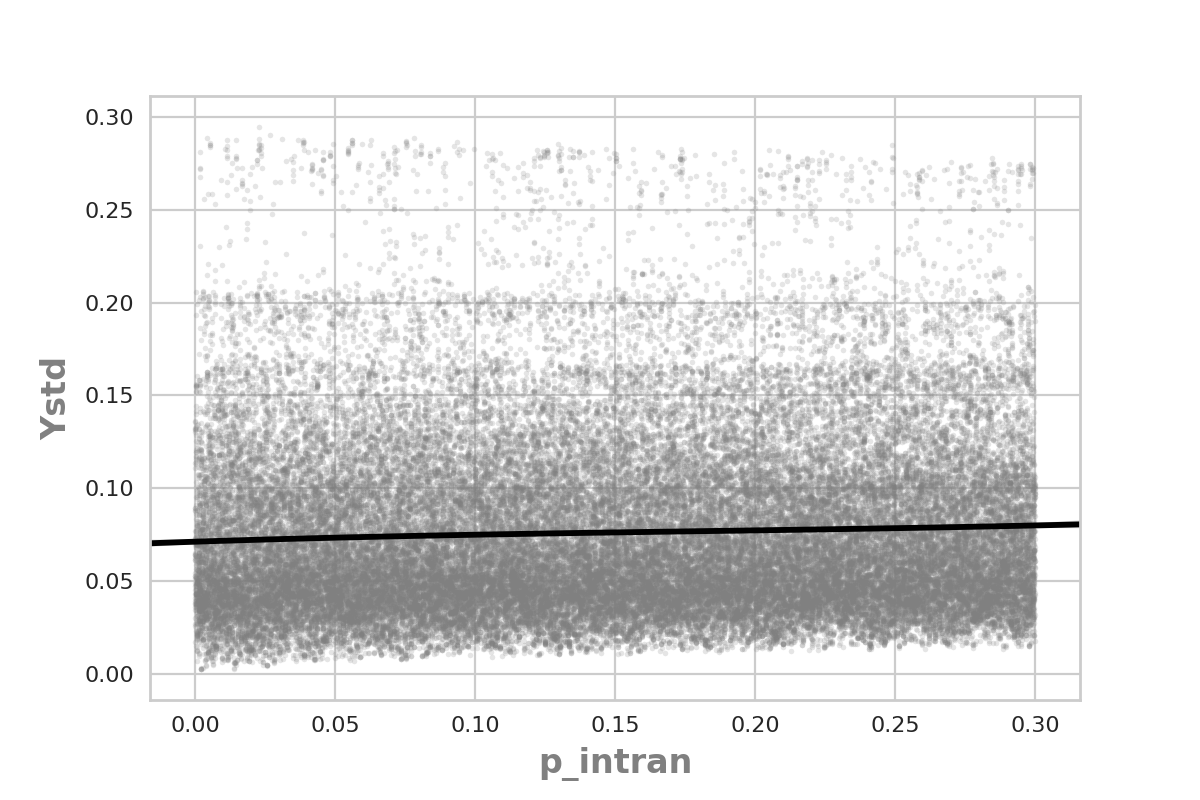
\includegraphics[width=\textwidth]{ims/nlregressions/nlregressionmutatingop_intran.png}
    \end{subfigure}
    
    \label{fig:scatter2}
    \source{Marcelo Veloso Maciel, 2018.}
  \end{figure}


%%% Local Variables:
%%% mode: latex
%%% TeX-master: "master"
%%% End:
